\documentclass[aspectratio=169,fleqn]{beamer}
\usepackage{spc}
\usepackage{graphicx}
\begin{document}

\begin{frame}
  \title{\vspace{-5ex}\darkblue Scoping the next stock assessment
    platform\\[2ex]
    \it\large\darkgray
    Project 123 progress update and outline of options}
  \author{\vspace{-10ex}\darkgray\bf
    Arni Magnusson, Nick Davies,\\[0.5ex]
    Graham Pilling, Paul Hamer}
  \date{\darkgreen SPC Pre-Assessment Workshop (PAW)\\[0.5ex]
    Nouméa, 9 April 2025}
  \titlepage
\end{frame}

% ______________________________________________________________________________

\begin{frame}{Overview}
  \begin{itemize}
    \item[] {\bf\darkblue Overall Plan} \comment{migrating from MFCL, project
      outline, objectives,\\
      \h{17.1ex}activities, timeline, required resources}\\[5ex]
    \item[] {\bf\darkblue SC20 in 2024} \comment{international expert meeting,
      overview of software,\\
      \h{18.5ex}identifying activities to prioritize}\\[5ex]
    \item[] {\bf\darkblue Latest Developments} \comment{workshop in Sep 2024,
      multiple-criteria decision analysis,\\
      \h{27ex}updated evaluation and advice, workshop in May 2025}\\[5ex]
    \item[] {\bf\darkblue SC21 in 2025} \comment{evaluation of model features,
      outline of options,\\
      \h{18.5ex}SPC staff positions \& consultants}\\[1ex]
  \end{itemize}
\end{frame}

% ______________________________________________________________________________

\begin{frame}{The need to to migrate to new software}
  \begin{itemize}
    \item[] MULTIFAN-CL (MFCL) has been used in SPC tuna assessments since
    1990s\\[4ex]
    \item[] MFCL team (Dave Fournier, John Hampton, Nick Davies) retiring in the
    2020s\\[4ex]
    \item[] Development of new features is slowing down\\[4ex]
    \item[] Resources are being allocated to succession plans\\[2ex]
  \end{itemize}
\end{frame}

% ______________________________________________________________________________

\begin{frame}{Migrating all MFCL assessments to other platforms}
  \textbf{\darkgreen Shared} process, {\darkgreen\bf continuous} communications,
  {\darkgreen\bf adaptive} strategy\\[2ex]
  \begin{itemize}
    \item[] {\blue\bf WCPFC} ~--~ guidance\\[2ex]
    \item[] {\blue\bf SPC} ~--~ conduct and coordinate the work\\[3ex]
  \end{itemize}
  Also involved: other tuna RFMOs and various research labs\\[4ex]
  Swordfish and striped marlin 2025 assessments migrating to Stock
  Synthesis\\[4ex]
  Tuna assessments currently in MFCL, evaluating alternative platforms\\
  and development options\\[1ex]
\end{frame}

% ______________________________________________________________________________

\begin{frame}{Project outline}
  This scoping project is scheduled from 1 Feb 2024 to 31 Dec 2026. It
  will:\\[3ex]
  \begin{itemize}
    \item[] Evaluate features and capabilities that will be important in future
    tuna assessments\\[3ex]
    \item[] Explore fitting models to tuna data using existing software
    platforms\\[3ex]
    \item[] Guide decisions on what kind of new software development will be
    required\\[3ex]
    \item[] Establish collaboration with tuna RFMOs and research labs to achieve
    these goals\\[3ex]
  \end{itemize}
\end{frame}

% ______________________________________________________________________________

\begin{frame}{Objectives}
  The ideal outcome would be that in 10--15 years, the WCPFC tuna assessments\\
  are conducted in software that has the following three characteristics or
  criteria:\\[1.5ex]
  \begin{enumerate}
    \item {\bf\blue Scientific quality}: has good estimation performance, makes
    good use\\
    of available data, allows spatial and temporal variability in processes,\\
    runs fast.\\[1.5ex]
    \item {\bf\blue Beginner friendly}: new staff scientists can conduct a stock
    assessment\\
    in their first year of contract, configuring and understanding the
    models.\\[1.5ex]
    \item {\bf\blue Widely used}: large development team and user community
    beyond SPC,\\
    new staff scientists can find expert help outside of SPC, tools
    to work\\
    with model input and output are feature complete and maintained
    outside\\
    of SPC, external reviewers have a good understanding of model\\
    configurations and options.\\[2ex]
  \end{enumerate}
\end{frame}

% ______________________________________________________________________________

\begin{frame}{2024 project activities}
  \begin{itemize}
    \item[] Scoping project launched (Feb)\\[3ex]
    \item[] PAW discussion (Mar)\\[3ex]
    \item[] International expert meeting (May--Jun)\\[3ex]
    \item[] SC20 discussion (Aug)\\[3ex]
    \item[] Developer workshop (Aug--Sep)\\[3ex]
    \item[] Follow up with tuna RFMOs and research labs (Dec)\\[2ex]
  \end{itemize}
\end{frame}

% ______________________________________________________________________________

\begin{frame}{2025 project activities}
  \begin{itemize}
    \item[] Evaluation of RTMB as a development platform (Jan--Feb)\\[3ex]
    \item[] PAW discussion (Apr)\\[3ex]
    \item[] Follow up with tuna RFMOs and research labs (Apr)\\[3ex]
    \item[] Spatio-temporal tagging model workshop (May)\\[3ex]
    \item[] SC21 discussion (Aug)\\[3ex]
    \item[] Model development workshop (Quarter 4)\\[2ex]
  \end{itemize}
\end{frame}

% ______________________________________________________________________________

\begin{frame}{2026 draft plan}
  \begin{itemize}
    \item[] Evaluation of external analysis of tagging data (Quarter 1)\\[2ex]
    \item[] PAW discussion (Apr)\\[2ex]
    \item[] Model development workshop (Quarter 2)\\[2ex]
    \item[] Follow up with tuna RFMOs and research labs (Quarter 2)\\[2ex]
    \item[] SC22 discussion, final report of P123 (Aug)\\[2ex]
    \item[] $\Rightarrow$ Launch a project similar to P123, {\green
      coordinating} activities related to\\
    \phantom{$\Rightarrow$} the migration of assessments and related research \&
    development\\[2ex]
    \item[] $\Rightarrow$ Launch collaborative projects {\green conducting} work
    related to the\\
    \phantom{$\Rightarrow$} development of next-generation assessment models\\[2ex]
  \end{itemize}
\end{frame}

% ______________________________________________________________________________

\begin{frame}{Scoping project (first line)\\[0.2ex]
    and possible follow-up projects (next lines)}
  ~\h{-3ex}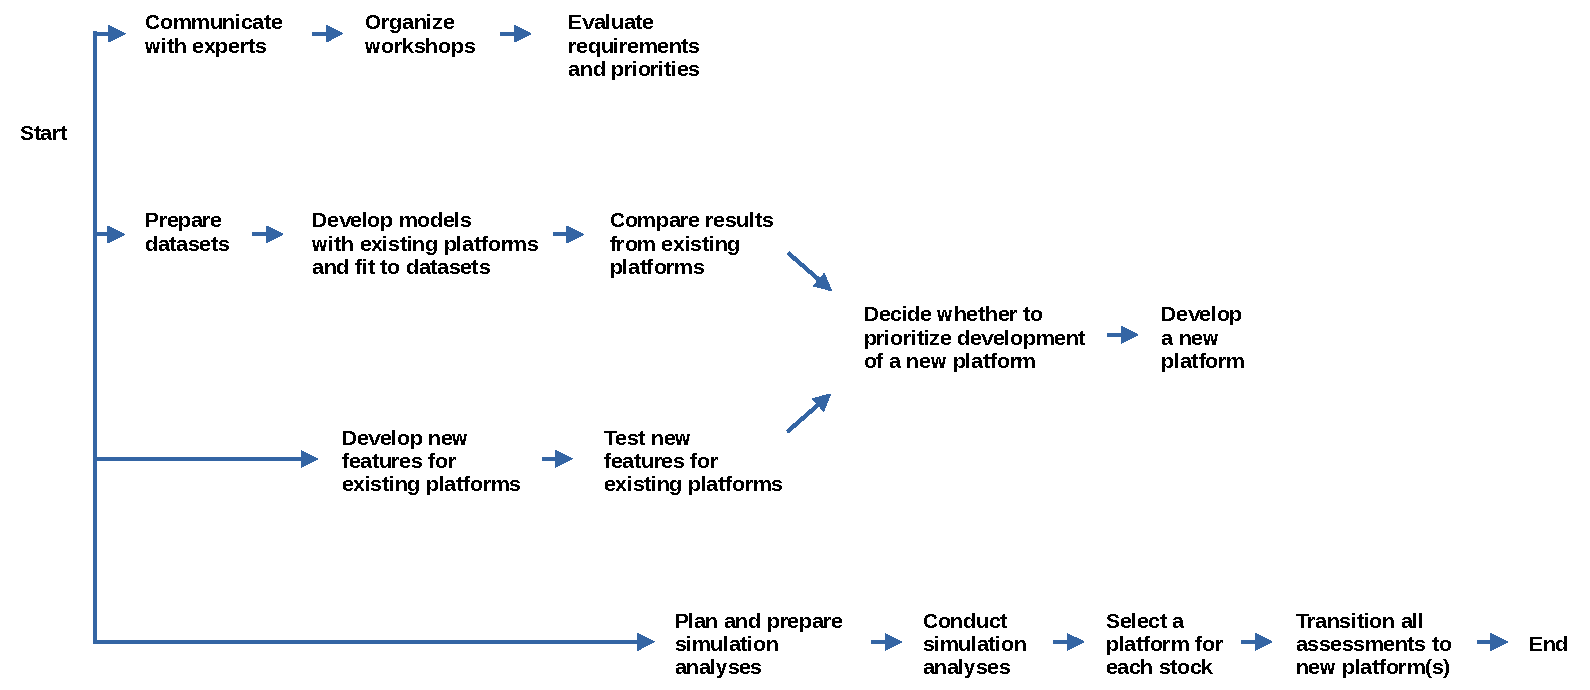
\includegraphics[width=1.05\textwidth]{p123_diagram}
\end{frame}

% ______________________________________________________________________________

\begin{frame}{Required resources}
  The overarching objective of transitioning all WCPFC assessments from
  MULTIFAN-CL\\[0.5ex]
  to other software platforms will require a larger project with
  additional project resources\\[0.5ex]
  beyond the standard service provision agreement for stock assessments, to
  allow some\\[0.5ex]
  staff to focus on model exploration and software development.
\end{frame}

% ______________________________________________________________________________

\begin{frame}{Collaboration with other tuna RFMOs}
  Other tuna RFMOs use primarily Stock Synthesis for tuna assessments,\\[0.5ex]
  a platform that is also expected to be phased out in the not-too-distant
  future.\\[0.5ex]
  Therefore, it would make sense for WCPFC and other tuna RFMOs to
  coordinate\\[0.5ex]
  and collaborate in software succession plans and new software
  development.\\[5ex]
  Ideally, each tuna RFMO could hire/assign one full-time person to the
  project\\[0.5ex]
  for 5 years, or until assessments have been transitioned to the new
  software.\\[4ex]
\end{frame}

% ______________________________________________________________________________

\begin{frame}{SPC staff positions and consultants}
  Compared to the other tuna RFMOs, there is greater urgency for WCPFC\\[0.5ex]
  to move this project forward.\\[4ex]

  Independent of decisions and commitments of the other tuna RFMOs, the\\[0.5ex]
  main project would probably require one staff to be dedicated to this
  work\\[0.5ex]
  initially and, depending on the direction taken, an additional staff or
  consultant\\[0.5ex]
  with software development skills.\\[4ex]

  It is likely that transitioning MFCL assessments to other software is at
  least\\[0.5ex]
  a 5 year proposition.\\[1ex]
\end{frame}

% ______________________________________________________________________________

\begin{frame}{Scientific quality and rate of progress}
  The resources committed to the main project will determine the\\[0.5ex]
  scientific quality of the end result and the number of years it takes\\[0.5ex]
  to transition all SPC assessments from MFCL to other platforms.\\[5ex]
  Now that the first author of MFCL, David Fournier, has retired, it would
  be\\[0.5ex]
  highly beneficial for the project to move relatively fast, before the
  remaining\\[0.5ex]
  MFCL team (John Hampton and Nick Davies) will retire and no longer be\\[0.5ex]
  available for consultation and involvement regarding software design,
  testing\\[0.5ex]
  and technical decisions.
\end{frame}

% ______________________________________________________________________________

\begin{frame}{Summary}
  \begin{itemize}
    \item[] {\bf\darkblue Overall Plan} \comment{migrating from MFCL, project
      outline, objectives,\\
      \h{17.1ex}activities, timeline, required resources}\\[5ex]
    \item[] {\bf\darkblue SC20 in 2024} \comment{international expert meeting,
      overview of software,\\
      \h{18.5ex}identifying activities to prioritize}\\[5ex]
    \item[] {\bf\darkblue Latest Developments} \comment{workshop in Sep 2024,
      multi-objective optimization,\\
      \h{27ex}updated advice and analysis, workshop in May 2025}\\[5ex]
    \item[] {\bf\darkblue SC21 in 2025} \comment{evaluation of model features,
      SPC staff positions \& consultants}\\[1ex]
  \end{itemize}
\end{frame}

% ______________________________________________________________________________

\begin{frame}{SC20 discussion}
  \begin{itemize}
    \item Whether SPC should migrate upcoming {\darkgreen\bf billfish
      assessments} to Stock Synthesis\\
    \comment{\gray swordfish 2025, striped marlin 2029}\\[4ex]
    \item Select {\darkgreen\bf scoping project} tasks to prioritize in
    2024--2026\\
    \comment{\gray from the list of 10 tasks in the report, or other
      tasks}\\[4ex]
    \item What is needed to launch the {\darkgreen\bf main project} and when\\
    \comment{\gray conducting model exploration and software development, TORs,
      resources}\\[3ex]
  \end{itemize}
\end{frame}

% ______________________________________________________________________________

\begin{frame}{Stock Synthesis}
  \textit{Cons}
  \begin{itemize}
    \item[--] expected to be phased out in the not-too-distant future\\[1ex]
    \item[--] fewer features than MFCL\\[3ex]
  \end{itemize}
  \textit{Pros}
  \begin{itemize}
    \item[+] used by IATTC, IOTC, ICCAT, and ISC (and NOAA, ICES, GFCM,
    etc.)\\[1ex]
    \item[+] facilitates collaboration between the tuna RFMOs, including future
    development\\[1ex]
    \item[+] shortens training time for new SPC staff, makes skills and
    experience transferable\\[1ex]
    \item[+] large user community, relevant for peer reviews and discussing
    technical decisions\\[1ex]
    \item[+] exceptionally complete suite of tools, diagnostics, automated plots
    and tables\\[1ex]
    \item[+] next-generation frameworks will support transitioning from Stock
    Synthesis\\[1ex]
  \end{itemize}
\end{frame}

% ______________________________________________________________________________

\begin{frame}{Recommendations from 2024 international expert meeting}
  \begin{enumerate}
    \item {\darkgreen\bf Tuna} assessment software\\
    \comment{\gray design and develop a model specific for tuna
      assessments}\\[1ex]
    \item {\darkgreen\bf RTMB} programming environment\\
    \comment{\gray lean software development paradigm, maybe a specific model
      for each species}\\[1ex]
    \item {\darkgreen\bf State-space} formulation\\
    \comment{\gray statistically and computationally efficient way to allow
      time-varying processes}\\[1ex]
    \item {\darkgreen\bf Age-length} structure\\
    \comment{\gray explicitly track the population by age and length, if not too
      costly}\\[1ex]
    \item {\darkgreen\bf Simple} models\\
    \comment{\gray short-term staff, young scientists, simple user interface,
      simpler models}\\[1ex]
    \item {\darkgreen\bf Collaboration} between tuna RFMOs\\
    \comment{\gray MFCL and Stock Synthesis in a sunset phase, data analyses
      comparable between RFMOs}\\[1.5ex]
  \end{enumerate}
\end{frame}

% ______________________________________________________________________________

\begin{frame}{Stock assessment software}
  Existing software, ready for multi-region tuna assessments\\[3ex]
  \begin{itemize}
    \item[-] {\darkgreen\bf Stock Synthesis} is used by IATTC, IOTC, and
    ICCAT\\[3ex]
    \item[-] {\darkgreen\bf Gadget} has many features relevant for tuna
    assessments\\[3ex]
    \item[-] {\darkgreen\bf Casal} has many features relevant for tuna
    assessments\\[4ex]
  \end{itemize}
  These could be extended further as needs arise\\[2ex]
\end{frame}

% ______________________________________________________________________________

\begin{frame}{Stock assessment software}
  Software that could be developed further:\\[3ex]
  \begin{itemize}
    \item[-] {\darkgreen\bf sbt} is built around CKMR, currently for
    single-region assessments\\[3ex]
    \item[-] {\darkgreen\bf ALSCL} is a state-space model that fits length
    comps, currently no catches\\[3ex]
    \item[-] {\darkgreen\bf WHAM$\,$\raisebox{0.15ex}{+}$\,$Length} is a
    state-space that fits length comps, currently single-region\\[3ex]
    \item[-] {\darkgreen\bf SAM$\,$\raisebox{0.15ex}{+}$\,$Length} is an early
    exploration of extending SAM to fit length comps\\[3ex]
    \item[-] {\darkgreen\bf Stock Synthesis$\,$\raisebox{0.15ex}{+}$\,$Enhanced
      Tags} is a proposed enhancement of the tag module\\[2ex]
  \end{itemize}
\end{frame}

% ______________________________________________________________________________

\begin{frame}{Stock assessment software}
  Also relevant:\\[4ex]
  \begin{itemize}
    \item[-] {\darkgreen\bf Stock Synthesis$\,$\raisebox{0.15ex}{+}$\,$CKMR} is
    an experimental add-on, not included in core software\\[4ex]
    \item[-] {\darkgreen\bf FIMS}, NOAA project coordinating the development of
    a next-generation framework\\[6ex]
  \end{itemize}
\end{frame}

% ______________________________________________________________________________

\begin{frame}{Possible tasks for SPC to prioritize}
  Subject to SC advice and funding approvals by WCPFC:\\[4ex]
  {\orange\it Migrate assessments to existing software}\\[2ex]
  \begin{enumerate}
    \item Move the {\darkgreen swordfish} assessment to Stock Synthesis\\
    \comment{\gray relatively simple compared to other SPC assessments}\\[3ex]
    \item Move the {\darkgreen striped marlin} assessment to Stock Synthesis\\
    \comment{\gray also relatively simple}\\[3ex]
  \end{enumerate}
  \gray stepwise: previous MFCL diagnostic $\Rightarrow$ catch-conditioned
  MFCL $\Rightarrow$ Stock Synthesis
\end{frame}

% ______________________________________________________________________________

\begin{frame}{Possible tasks for SPC to prioritize}
  Subject to SC advice and funding approvals by WCPFC:\\[3.5ex]
  {\orange\it Model exploration using existing software}\\[2ex]
  \begin{enumerate}\setcounter{enumi}{2}
    \item Explore Casal/Gadget/Stock Synthesis/sbt models for {\darkgreen
      albacore}\\
    \comment{\gray simpler than the other tuna species}\\[3ex]
    \item Explore Casal/Gadget/Stock Synthesis models for original {\darkgreen
      five-region yellowfin} data\\
    \comment{\gray test capabilities of platforms: regions, tags, large number
      of fisheries}\\[3ex]
    \item Explore a variety of models for a simplified {\darkgreen single-region
      yellowfin} tuna dataset\\
    \comment{\gray ALSCL, Casal, Gadget, MFCL, sbt, Stock Synthesis,
      WHAM\raisebox{0.15ex}{+}Length}\\[3ex]
  \end{enumerate}
\end{frame}

% ______________________________________________________________________________

\begin{frame}{Possible tasks for SPC to prioritize}
  Subject to SC advice and funding approvals by WCPFC:\\[3ex]
  {\orange\it Extend existing software}\\[1.5ex]
  \begin{enumerate}\setcounter{enumi}{5}
    \item ALSCL$\,$\raisebox{0.15ex}{+}$\,$Fleets\\
    \comment{\gray Fan Zhang (Shanghai Ocean University) and Nick Davies (SPC
      consultant)}\\[1.5ex]
    \item Stock Synthesis$\,$\raisebox{0.15ex}{+}$\,$Enhanced Tags\\
    \comment{\gray Nicholas Ducharme-Barth, Matthew Vincent (NOAA), and Arni
      Magnusson (SPC)}\\[1.5ex]
    \item WHAM$\,$\raisebox{0.15ex}{+}$\,$Length\\
    \comment{\gray Giancarlo Correa (AZTI) and Arni Magnusson (SPC)}\\[1.5ex]
    \item SAM$\,$\raisebox{0.15ex}{+}$\,$Length\\
    \comment{\gray Anders Nielsen (DTU), Colin Millar (ICES), and Arni Magnusson
      (SPC)}\\[1.5ex]
  \end{enumerate}
\end{frame}

% ______________________________________________________________________________

\begin{frame}{Possible tasks for SPC to prioritize}
  Subject to SC advice and funding approvals by WCPFC:\\[4ex]
  {\orange\it Design and develop new software for tuna assessments}\\[2ex]
  \begin{enumerate}\setcounter{enumi}{9}
    \item Initial explorations using {\darkgreen RTMB}\\
    \comment{\gray Nick Davies (SPC consultant) and Arni Magnusson (SPC)}
  \end{enumerate}
\end{frame}

% ______________________________________________________________________________

\begin{frame}{Possible tasks for SPC to prioritize}
  \begin{enumerate}
    \item Move the {\darkgreen swordfish} assessment to Stock Synthesis\\[1ex]
    \item Move the {\darkgreen striped marlin} assessment to Stock
    Synthesis\\[1ex]
    \item Explore Casal/Gadget/Stock Synthesis/sbt models for {\darkgreen
      albacore}\\[1ex]
    \item Explore Casal/Gadget/Stock Synthesis models for original {\darkgreen
      five-region yellowfin} data\\[1ex]
    \item Explore a variety of models for a simplified {\darkgreen single-region
      yellowfin} tuna dataset\\[1ex]
    \item ALSCL$\,$\raisebox{0.15ex}{+}$\,$Fleets\\[1ex]
    \item Stock Synthesis$\,$\raisebox{0.15ex}{+}$\,$Enhanced Tags\\[1ex]
    \item WHAM$\,$\raisebox{0.15ex}{+}$\,$Length\\[1ex]
    \item SAM$\,$\raisebox{0.15ex}{+}$\,$Length\\[1ex]
    \item Initial explorations using {\darkgreen RTMB}\\[1ex]
  \end{enumerate}
\end{frame}

% ______________________________________________________________________________

\begin{frame}{Project website}
  \centering\small
  \textblue{\url{https://github.com/PacificCommunity/ofp-sam-transition-plan}}
\end{frame}

\end{document}
